% !TeX spellcheck = cs_CZ
%{\tikzset{external/prefix={tikz/FYZI/}}
% \tikzset{external/figure name/.add={ch10_}{}}
%---------------------------------------------------------------------------------------------------
% file fey1ch12.tex
%---------------------------------------------------------------------------------------------------
%================ Kapitola 12: Charakteristiky síly ================================================
\chapter{Charakteristiky síly}\label{fyz:IchapXII}
\minitoc
  \section{Co je to síla?}\label{fyz:IchapXIIsecI}
    I když je studium fyzikálních zákonů zajímavé a vyplatí se už prostě proto, že nám pomáhá 
    chápat a využívat přírodu, je třeba se čas od času zastavit a položit si otázku \uv{Jaký je 
    jejich skutečný smysl?} Hledání smyslu jakéhokoli výroku je od nepaměti předmětem zájmu 
    filozofů a hledání smyslu fyzikálních zákonů je ještě zajímavější, neboť obecně se věří, že 
    tyto zákony reprezentují určitý druh reálného poznání. Význam poznání je hluboký filozofický 
    problém a ptát se „Co to znamená?“, je vždy důležité.
    
    Zeptejme se: „Co znamená Newtonův zákon, který píšeme jako \(\vec{F}=m \vec{a}\,\)? Jaký smysl 
    má síla, hmotnost a zrychlení?“ Smysl hmotnosti jsme schopni intuitivně chápat a zrychlení 
    dokážeme \emph{definovat}, jestliže chápeme smysl polohy a času. Těmto věcem se nebudeme 
    věnovat, ale soustředíme se na to, co je to síla. Odpověď je stejně jednoduchá: „Když těleso 
    zrychluje, působí na něho nějaká síla“. To nám říká Newtonův zákon, takže nejpřesnější a 
    nejkrásnější definicí síly může být prostě to, že řekneme, že síla je hmotnost tělesa násobená 
    zrychlením. Předpokládejme, že je-li součet všech vnějších sil roven nule, platí zákon 
    zachování hybnosti. Pak vzniká otázka: „Co to \emph{znamená}, že součet všech vnějších sil je 
    roven nule“. Tady nemůže být něco v pořádku, neboť tento výrok neříká nic nového. Jestliže jsme 
    objevili základní zákon, podle něhož je síla rovna součinu hmotností a zrychlení, a pak 
    definujeme sílu jako hmotnost krát zrychlení, neobjevili jsme nic nového. Sílu bychom mohli 
    \emph{definovat} i tak, že nepůsobí-li na těleso žádná síla, těleso se nadále pohybuje po 
    přímce s konstantní rychlostí. Jestliže pak zpozorujeme, že těleso se \emph{nepohybuje} po 
    přímce s konstantní rychlostí, můžeme říci, že na něj působí síla. Takováto tvrzení nemohou 
    tvořit obsah fyziky, neboť jsou to definice v kruhu. Uvedená newtonovská definice se zdá být 
    takovou nejpřesnější definicí síly, která apeluje na matematiky, přesto je zcela neužitečná, 
    neboť z takovéto definice nelze získat vůbec žádnou předpověď. Mohli bychom celý den sedět v 
    křesle a vytvářet si definice podle libovůle, ale zjistit, co se stane, když se srazí dvě 
    koule, nebo když se závaží zavěsí na strunu, je zcela jiná věc, neboť \emph{chování} těles 
    nelze vyjádřit žádnými definicemi.
    
    Například, těleso odkázané samo na sebe si zachovává svou polohu a nepohybuje se. Když pak 
    uvidíme, že se něco pohybuje, můžeme si vymyslet nové slovo a říct, že to způsobuje třeba 
    „zíla\footnote{V originále slovní hříčka force-gorce.}“. „Zíla“ je rychlost změny polohy. Máme 
    tedy pěkný zákon - vše setrvává v klidu, kromě případu, kdy působí nějaká „zíla“. Vidíme, že by 
    to byla analogická definice k uvedené definici síly a neobsahovala by žádnou informaci. 
    Skutečný obsah Newtonových zákonů je, že navíc k zákonu \(\vec{F}= m\vec{a}\) by měla mít síla 
    ještě nějaké \emph{nezávislé vlastnosti}, ale tyto \emph{specifické} nezávislé vlastnosti síly 
    nebyly zcela popsány Newtonem, ani nikým jiným, a proto je fyzikální zákon \(\vec{F}= 
    m\vec{a}\) neúplný. Z toho vyplývá, že studujeme-li součin hmotnosti a zrychlení, přičemž ho 
    nazveme silou, tj. studujeme charakteristiky síly jako předmět našeho zájmu, zjistíme, že síly 
    se vyznačují určitou jednoduchostí; zákon tvoří dobrý program pro analýzu přírody, je náznakem 
    toho, že síly budou jednoduché.
    
    Prvním příkladem takovýchto sil byl úplný Newtonův gravitační zákon a při formulování tohoto 
    zákona odpovídal Newton na otázku „Co je to síla?“. Kdyby neexistovalo nic jiného než 
    gravitace, tvořila by kombinace tohoto zákona se zákonem síly (druhým pohybovým zákonem) úplnou 
    teorii. Kromě gravitace však existuje mnoho jiného a my chceme použít Newtonovy zákony v mnoha 
    různých situacích. Proto, abychom se dostali dále, musíme něco říci o vlastnostech síly.
    
    Například, hovoříme-li o síle, vždy se mlčky předpokládá, že nejsou-li přítomna fyzikální 
    tělesa, je síla vždy rovna nule. Najdeme-li nenulovou sílu, najdeme někde nablízku ještě něco, 
    co je zdrojem této síly. Tento předpoklad se zcela liší od případu již výše uvedené „zíly“. 
    Jednou z nejdůležitějších charakteristik síly je její materiální původ a to \emph{není} jen 
    definice.
    
    Newton měl ještě jedno pravidlo týkající se sil: síly mezi interagujícími tělesy jsou stejně 
    velké a opačné - akce je rovna reakci. Ukazuje se, že toto pravidlo neplatí zcela přesně. Ani 
    zákon \(\vec{F}= m\vec{a}\) neplatí zcela přesně; kdyby byl definicí, museli bychom říci, že 
    \emph{vždy} platí zcela přesně, ale není tomu tak.
    
    Můžete namítnout: „Tato nepřesnost se mi nelíbí, měl bych rád všechno exaktně definováno; v 
    některých knihách se říká, že jen taková věda je exaktní vědou, v níž je vše předefinováno“. 
    Trváme-li na přesné definici síly, nikdy ji nedostaneme! Za prvé, protože Newtonův druhý zákon 
    neplatí přesně, za druhé, k pochopení fyzikálních zákonů je třeba pochopit i to, že všechny 
    jsou určitou aproximací.
    
    Každá jednoduchá idea je přiblížením. Pro ilustraci si vezměme nějaký předmět... Co je to 
    předmět? Filozofové vždy řeknou: „No, například křeslo“. V okamžiku, kdy to řeknou, je jasné, 
    že nevědí o čem hovoří. Co jeto křeslo? Křeslo je určitá věc tamto… Určitá?, jak určitá? Čas od 
    Času se z něj vypařují atomy - ne mnoho, několik - padá na ně prach a rozpouští se v nátěru; 
    takže podat přesnou definici křesla, přesně říci, které atomy jsou křesla a které jsou vzduch 
    nebo které atomy jsou prach, které atomy jsou nátěr křesla - to je nemožné. Takže hmotnost 
    křesla lze definovat jen přibližně. Stejně tak není možné definovat hmotnost jednotlivého 
    předmětu, neboť ve světě neexistují žádné jednotlivé, osamocené předměty - každý je smíšeninou 
    mnoha věcí, takže vždy máme co činit s řadou přiblížení a idealizací.
    
    Celý trik spočívá v idealizaci. Ve velmi dobrém přiblížení (snad 1 ku \num{e10}) se počet atomů 
    křesla za minutu nezmění a nejsme-li příliš přesní, můžeme si křeslo zidealizovat jako určitou 
    věc. Stejně tak můžeme pomocí idealizace poznávat charakteristiky síly, nejsme-li příliš 
    přesní. Můžeme být nespokojeni s přibližným pohledem na přírodu, o nějž se pokouší fyzika (vždy 
    se snaží o zvýšení přesnosti dané aproximace) a můžeme dát přednost matematické definici, ale 
    matematické definice nemohou nikdy fungovat v reálném světě. Matematická definice bude dobrá 
    pro matematiky, kde lze sledovat celou logiku, ale fyzikální svět je složitý. To jsme naznačili 
    na více příkladech, jako byly vlny v oceánu nebo pohár vína. Jestliže se pokoušíme tento svět 
    dělit na izolované části, například víno a pohár, a jestliže se snažíme hovořit o hmotnosti 
    jedné z nich, jak můžeme vědět, co je co, když jedno se rozpouští v druhém? Již síly, působící 
    na jednotlivé věci, obsahují přiblížení a jakýkoli systém názorů na reálný svět, aspoň dnes, 
    musí obsahovat nějaké přiblížení.
    
    Tento systém se zcela liší od systému matematiky, kde lze všechno definovat a pak 
    \emph{nevíme}, o čem je vlastně řeč. Skutečně, sláva matematiky spočívá v tom, že v ní 
    \emph{nemusíme říci, o čem hovoříme}. Její sláva spočívá v tom, že její zákony, důkazy a logika 
    jsou nezávislé na tom, co „to“ je. Kdybychom měli jakoukoli jinou množinu předmětů, jež 
    vyhovuje axiomům euklidovské geometrie, když vytvoříme nové definice a použijeme správnou 
    logiku, budou správné i všechny důsledky, bez ohledu na to, jaké to byly předměty. 
    Nakreslíme-li však v přírodě přímku, nebo jí vytvoříme pomocí světelného paprsku a teodolitu, 
    jak se to dělá při mapování, je to přímka v euklidovském smyslu? Ne, děláme určitou aproximaci; 
    nitkový kříž má určitou šířku, ale geometrická přímka nemá žádnou šířku, takže otázka, zda je, 
    nebo není euklidovská geometrie vhodná k mapování, to je fyzikální a ne matematická otázka! 
    Avšak z experimentálního hlediska, ne z hlediska matematiky, potřebujeme vědět, zda se 
    Euklidovy zákony vztahují na takovou geometrii, kterou používáme při mapování; vyslovíme proto 
    hypotézu, že ano, což celkem dobře souhlasí. Není to však přesné, neboť naše mapovací přímky 
    nejsou skutečnými matematickými přímkami. Zda euklidovské přímky, jež jsou ve skutečnosti 
    abstraktní, souvisí s přímkami, které používáme, to je otázka zkušeností a nelze ji zodpovědět 
    pouhým uvažováním.
    
    Podobně, \(\vec{F}= m\vec{a}\) nemůžeme prostě nazvat definicí síly, dedukovat všechno čistě 
    matematicky, a z mechaniky udělat matematickou teorii, když mechanika popisuje přírodu. Pomocí 
    vhodných postulátů lze vždy sestrojit matematický systém, jak to provedl Euklidés, ale nemůžeme 
    vytvořit matematiku přírody, neboť dříve či později, musíme zjistit, zda naše axiomy platí pro 
    reálné přírodní objekty. Takto se bezprostředně dostáváme ke komplikovaným a „špinavým“ 
    přírodním objektům, ale pomocí stále se zpřesňujících aproximací.
    
  \section{Tření}\label{fyz:IchapXIIsecII}
    Předcházející úvahy ukazují, že ke skutečnému pochopení Newtonových zákonů je třeba diskuze o 
    silách. Cílem této kapitoly je uvést takovou diskuzi jako určité dovršení Newtonových zákonů. 
    Definici zrychlení a toho, co s ní souvisí, jsme již probrali; nyní je třeba se věnovat studiu 
    vlastností síly. Tato kapitola, na rozdíl od předcházející, nebude řešit problémy příliš 
    detailně, neboť síly jsou dost složité.
    
    Abychom začali s konkrétní silou, vezměme sílu, jež brzdí letadlo při letu vzduchem. Jaký je 
    zákon této síly? Pro každou sílu určitě existuje zákon, takže nějaký \emph{musíme najít}. 
    Člověk by si těžko pomyslel, že by zákon takové síly byl jednoduchý. Představme si, co brzdí 
    letadlo při jeho letu  vzduchem - vzduch obtékající křídla, víření za letadlem, změny proudění 
    vzduchu podél trupu i mnohé jiné komplikace a vidíme, že to nebude jednoduchý zákon. Na druhé 
    straně je pozoruhodný fakt, že síla brzdící letadlo je přibližně rovna konstantě násobené 
    rychlostí umocněnou na druhou, tedy \(F\sim cv^2\).
    
    Jaké postavení má takovýto zákon? Není analogický s \(\vec{F}= m\vec{a}\)? Vůbec ne, neboť 
    tento zákon je v první řadě empirickou záležitostí, získanou zhruba pomocí zkoušek v 
    aerodynamickém tunelu. Řekněme: „Dobře, ale \(F=ma\) může být i empirický zákon.“ To není 
    důvod, proč by mezi nimi neměl být rozdíl. Tento rozdíl nespočívá v tom, že je to empirický 
    zákon, ale v tom, jak chápeme přírodu - tento zákon je výsledným projevem celého komplexu jevů 
    a ne v podstatě jedné věci. Čím více ho budeme zkoumat, čím přesněji budeme měřit, tím bude 
    \emph{komplikovanější} a nikoli jednodušší. Jinými slovy, stále podrobnějším studiem zákona 
    brzdění letadla zjistíme, že je „chybnější" a „chybnější", a čím hlouběji se jím zabýváme, čím 
    přesněji měříme, tím se pravda stává komplikovanější - takže v tom smyslu ho nepovažujeme za 
    výsledek jednoduchého fundamentálního procesu, což souhlasí s naším původním předpokladem. 
    Například, při velmi malé rychlosti, tak malé, že letadlo neletí, ale je třeba pomalu taženo 
    vzduchem, změní se zákon brzdění a brzdné tření závisí na rychlosti spíše lineárně. Dalším 
    příkladem je brzdné tření při pomalém pohybu kuličky, bubliny nebo čehokoli jiného, ve viskózní 
    kapalině jako je med, kde je tření úměrné rychlosti, ale při rychlém pohybu, kdy za tělesem 
    vznikají víry (med nevíří, ale voda a vzduch ano), se stává přímo úměrným druhé mocnině 
    rychlosti (\(F=cv^2\)) a při dalším zvyšování rychlosti začíná selhávat i tento zákon. Ti, co 
    řeknou, že dochází k malé změně koeficientu úměrnosti, se chtějí vyhnout problému. Jsou tu však 
    ještě další velké komplikace, jež souvisí s tím, zda sílu působící na letadlo lze rozdělit na 
    sílu působící na křídla, sílu působící na přední část letadla atd. Ano, toto lze skutečně 
    provést, jestliže se zajímáme o napětí jednotlivých částí, ale pak musíme dostat speciální 
    zákony pro sílu na křídlech a podobně. Je zajímavé, že síla působící na jedno křídlo, závisí na 
    přítomnosti druhého křídla, tedy, kdybychom letadlo rozebrali a ve vzduchu nechali jen jedno 
    křídlo, nebude tato síla stejná, jako když je letadlo celé. Je to způsobeno tím, že část větru, 
    která naráží na přední část, se dostává až ke křídlům a změní sílu, jež na ně působí. Zdá se, 
    že je to zázrak, že tu platí tak jednoduchý, přibližný, empirický zákon, použitelný při 
    konstrukci letadel. Tento zákon však není toho druhu jako \emph{základní zákony} fyziky a čím 
    více ho studujeme, tím je komplikovanější. Studium závislosti koeficientu \(c\) na tvaru přední 
    části letadla je, mírně řečeno, beznadějné. Jednoduchý zákon k určení tohoto koeficientu v 
    závislosti na tvaru letadla ani neexistuje. Naopak, zákon gravitace je jednoduchý a jeho další 
    studium jen potvrzuje jeho skutečnou jednoduchost.
    
    Dosud jsme hovořili o dvou druzích tření: o tření, jež vzniká při rychlém pohybu ve vzduchu a 
    při pomalém pohybu v medu. Existuje i jiný druh tření, tzv. suché nebo \textbf{smykové tření}, 
    jež vzniká při smýkání jednoho tuhého tělesa po druhém. K udržení pohybuje v tomto případě 
    potřebná síla. Původ síly smykového tření - i to je velmi komplikovaná záležitost. Obě styčné 
    plochy jsou na úrovni atomů nepravidelné. Existuje mnoho styčných bodů, kde se atomy jakoby 
    silně navzájem přidržují a pak při smyku se od sebe odtrhnou, čímž vznikají vibrace. Tak nějak 
    to musí probíhat.
    
    \begin{figure}[ht!]  %\ref{fyz:fig121}
      \centering
      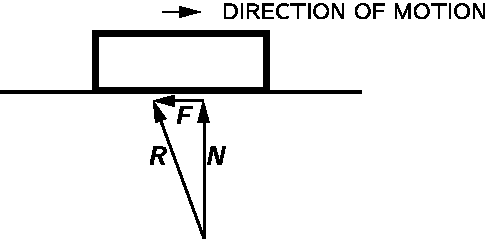
\includegraphics[width=0.7\linewidth]{fyz_fig121.pdf}
      \caption{Vztah mezi silou tření a kolmou silou při smýkání
              (\cite[s.~173]{Feynman01})}
      \label{fyz:fig121}
    \end{figure}
    Dříve se předpokládalo, že mechanizmus tohoto tření je velmi jednoduchý - že plochy obsahují 
    plno nerovností a že původ tření spočívá v překonávání takovýchto hrbolů. To však není možné, 
    neboť při takovém procesu by nedocházelo ke ztrátám energie. Ve skutečnosti však dochází ke 
    spotřebě energie. Mechanizmus ztráty energie je takový, že při smýkání po hrbolech se tyto 
    deformují, čímž v obou tělesech vzniknou kmity, pohyby atomů a po chvíli teplo. Opět je 
    pozoruhodné to, že toto tření lze empiricky popsat jednoduchým zákonem. Tento zákon říká, že 
    síla, potřebná k překonání tření při smýkání jednoho tělesa po druhém, závisí na síle kolmé k 
    povrchu, v němž se obě tělesa dotýkají. Opravdu, ve velmi dobrém přiblížení platí, že síla 
    tření je úměrná kolmé síle se skoro konstantním koeficientem. Platí
    \begin{equation}\label{FYZ:eq169}
      \boxed{F = \mu N}\,.
    \end{equation}
    kde \(\mu\) je \textbf{koeficient smykového tření} (obr. \ref{fyz:fig121}). Ačkoli tento 
    koeficient není roven přesně konstantě, je to dobrý empirický vztah, jenž slouží k přibližnému 
    určení síly tření pro potřeby inženýrské praxe. Pro příliš velkou kolmou sílu nebo příliš 
    velkou rychlost tento zákon selhává v důsledku nadměrného množství vytvářeného tepla. Je 
    důležité si uvědomit, že každý z těchto empirických zákonů má svá omezení, mimo nichž přestává 
    platit.
    
    Přibližnou správnost vztahu \(F = \mu N\) lze ukázat pomocí jednoduchého experimentu. Máme 
    například rovinu nakloněnou pod malým úhlem \(\vartheta\)? a položíme na ni kvádr s tíhou \(W\) 
    Potom zvětšujeme úhel nakloněné roviny, dokud se kvádr vlivem vlastní tíhy nezačne smýkat. 
    Složka síly směrem dolů podél roviny je \(W\sin\vartheta\). Ta se v případě, že se kvádr 
    pohybuje rovnoměrně, musí rovnat síle tření \(F\). Složka kolmá k rovině je \(W\cos\vartheta\), 
    což je kolmá síla \(N\). Pro tyto hodnoty platí vztah \(W\sin\vartheta = \mu W\cos\vartheta\), 
    odkud máme \(\mu = \sin\vartheta/\cos\vartheta = \tan\vartheta\). Kdyby tento zákon platil 
    přesně, těleso by se začalo smýkat při určitém úhlu. Zatížíme-li kvádr zvláštním závažím, pak 
    ačkoli se \(W\) zvětší, všechny síly vystupující v našem vztahu se zvětší v témž poměru a tíha 
    \(W\) se vykrátí. Je-li \(\mu\) konstantní, zatížený kvádr se začne pohybovat při stejném 
    sklonu. Při zkusmém určování úhlu \(\vartheta\) s původním zatížením zjistíme, že při zvětšení 
    závaží se kvádr začne smýkat opět při stejném sklonu. To platí i tehdy, kdy se závaží v 
    porovnání s původním závažím mnohonásobně zvětší. Z toho vyplývá, že koeficient tření nezávisí 
    na hmotnosti tělesa.
    
    V tomto experimentuje pozoruhodné, že je-li sklon roviny přibližně roven správnému úhlu 
    \(\vartheta\), nesmýká se kvádr rovnoměrně, ale zastavuje se. Na jednom místě se může zastavit 
    a na jiném se může pohybovat zrychleně. Takový pohyb nasvědčuje tomu, že koeficient tření je 
    jen přibližně konstantní a na rovině se mění od místa k místu. Takový pohyb nastane bez ohledu 
    na to, zda je kvádr zatížen nebo ne. Tyto změny jsou způsobeny různým stupněm drsnosti roviny 
    nebo snad špínou, rzí nebo cizími tělísky. Tabulky hodnot \(\mu\) pro „ocel na oceli“, „měď na 
    mědi“ apod. jsou všechny špatné, neboť ignorují faktory, o nichž jsme se právě zmiňovali, a jež 
    jsou pro správné určení \(\mu\) rozhodující. Tření „měď na měď“ je vlastně třením nečistot na 
    povrchu mědi.
    
    V experimentech popsaného typu tření téměř nezávisí na rychlosti. Mnozí věří, že tření, jež je 
    třeba překonat, abychom předmět uvedli do pohybu (statické tření), je mnohem větší než síla, 
    potřebná k udržení pohybu (smykové tření), ale jsou-li kovy suché, je velmi obtížné určit 
    nějaký rozdíl. Takový názor vznikl pravděpodobně na základě zkušeností s třením za přítomnosti 
    oleje nebo mazadla, nebo například, když byla tělesa přidržována pružinami nebo nějakými 
    pružnými podpěrkami, takže vznikla vazba.
    
    Provést přesné kvantitativní experimenty s třením je dost obtížné a zákony tření stále nejsou 
    zcela dobře prozkoumány navzdory mimořádné technické hodnotě takové přesné analýzy. Ačkoli 
    zákon \(F= \mu N\) platí dost přesně pro povrchy se standardní úpravou, důvod proč má zákon 
    právě takovouto formu, není zcela znám. Abychom ukázali, že koeficient y téměř nezávisí na 
    rychlosti, je třeba jemného experimentování, neboť zdánlivé tření se silně zmenší, jestliže 
    spodní povrch velmi rychle vibruje. V experimentech při velmi vysokých rychlostech je třeba 
    dbát, aby tělesa navzájem nevibrovala, neboť při velkých rychlostech se tření často zdánlivě 
    zmenší právě v důsledku vibrací. Zákon tření je rozhodně další z poloempirických zákonů, které 
    důkladně neznáme a je překvapující, bereme-li v úvahu všechnu vynaloženou námahu, že jsme 
    nedokázali tento jev lépe pochopit. V současnosti je opravdu takový stav, že teoretickou úvahou 
    neumíme koeficient tření mezi dvěma látkami ani odhadnout.
    
    Již jsme uvedli, že pokusy změřit \(\mu\) pomocí tření čistých látek, jako mědi po mědi, dají 
    falešné výsledky, neboť dotykové plochy nejsou z čisté mědi, ale obsahují různé oxidy a jiné 
    nečistoty. Když se pokusíme získat absolutně čistou měď, když vyčistíme a vyleštíme dotykové 
    plochy, necháme materiál odplynovat ve vakuu a provedeme všechna možná bezpečnostní opatření, 
    která nás jen napadnou, stále nedostaneme \(\mu\), neboť nakloníme-li zařízení třeba do 
    vertikální polohy, vrchní kvádr neodpadne - oba kusy mědi zcela přilnou! Koeficient \(\mu\), 
    jenž je menší než jedna pro poměrně tvrdé povrchy, se zvětší na několik jednotek! Důvodem 
    takovéhoto neočekávaného chování je, že všechny stýkající se atomy jsou stejného druhu a 
    nemohou rozeznat, že patří různým kusům mědi. Jsou-li mezi kovy jiné atomy, atomy oxidů, 
    mazadel a složitějších kontaminovaných povrchových vrstev, atomy „vědí“, že nepatří do stejného 
    tělesa. Když si uvědomíme, že jsou to právě síly působící mezi atomy, jež drží měď pohromadě 
    jako tuhé těleso, mělo by nám být jasné, že najít správný koeficient tření pro čisté kovy je 
    nemožné.
    
    Stejný úkaz můžeme pozorovat, když provedeme jednoduchý domácí experiment se skleněnou deskou a 
    skleněným pohárem. Pohár postavíme na sklo a posunujeme ho pomocí smyčky vlákna. Smýká se 
    poměrně dobře a lze cítit koeficient tření. Je nepravidelný, ale přece je to koeficient. Když 
    desku i spodek poháru navlhčíme, zjistíme, že se lepí, a když se dobře podíváme, najdeme na 
    skle škrábance, protože voda dokáže odstranit mastnotu i jiné nečistoty, takže potom máme 
    skutečně kontakt sklo na sklo. Tento kontakt je dobrý, pevně drží a klade rozdělení takový 
    odpor, že se sklo vytrhává, vznikají škrábance.
    
    
  \section{Molekulové síly}\label{fyz:IchapXIIsecIII}
    Dále se budeme zabývat charakteristikami molekulových sil. Jsou to síly mezi atomy a jsou 
    základním zdrojem tření. Na základě klasické fyziky nebyly molekulové síly nikdy uspokojivě 
    vysvětleny. K jejich plnému pochopení je třeba kvantové mechaniky. Empiricky zjištěná síla mezi 
    dvěma atomy je schematicky ilustrována na obr. \ref{fyz:fig122}, kde je znázorněna jako funkce 
    vzdálenosti \(r\) mezi nimi. Existují různé případy: například, v molekule vody jsou záporné 
    náboje posunuty k atomu kyslíku a střední polohy záporných a kladných nábojů nejsou ve stejném 
    bodě. Na jinou blízkou molekulu vody tak působí relativně velká síla, které se říká 
    \textbf{dipól} - \emph{dipólová síla}. Mnohé jiné systémy však mají náboje mnohem lépe 
    vyváženy, například molekuly kyslíku jsou plně symetrické. V tom případě, i když jsou záporné a 
    kladné náboje rozloženy po celé molekule, středy rozložení kladných a záporných nábojů jsou 
    totožné. Molekula, v níž nejsou tyto středy totožné, se nazývá \textbf{polární molekulou} a 
    součin náboje a vzdálenosti mezi těmito středy se nazývá \textbf{dipólový moment}. 
    \textbf{Nepolární molekulou} je taková molekula, pro níž jsou středy rozložení nábojů totožné. 
    Ukazuje se však, že u nepolárních molekul, v nichž jsou všechny elektrické síly neutralizovány, 
    na ně při velkých vzdálenostech působí přitažlivá síla, která se mění nepřímo úměrně sedmé 
    mocnině vzdálenosti, tedy \(F=k/r^7\), kde konstanta \(k\) závisí na druhu molekul. Proč je 
    tomu tak, to se dozvíme až při studiu kvantové mechaniky. Jde-li o dipóly, jsou síly větší. 
    Když se atomy nebo molekuly příliš přiblíží, odpuzují se velikou silou. Tato síla způsobuje, že 
    nepropadneme podlahou!
    
    \begin{figure}[ht!]  %\ref{fyz:fig122}
      \centering
      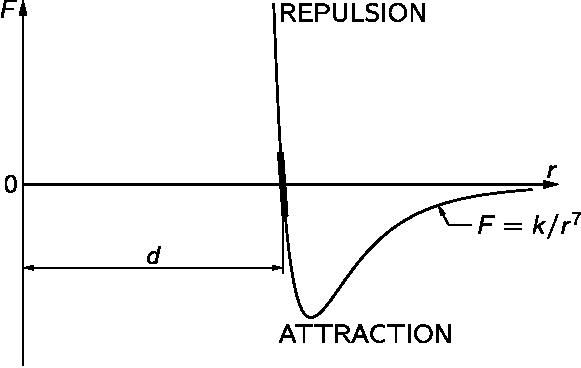
\includegraphics[width=0.7\linewidth]{fyz_fig122.pdf}
      \caption{Síla působící mezi dvěma atomy jako funkce jejich vzdálenosti 
              (\cite[s.~174]{Feynman01})}
      \label{fyz:fig122}
    \end{figure}
    Molekulové síly lze poměrně snadno demonstrovat; jedním způsobem je experiment s třením 
    skleněného poháru; jiným jsou dva zabroušené, velmi přesně rovné povrchy, které lze velmi těsně 
    přiblížit. Příkladem takových povrchů jsou Johanssonovy měrky, jež se používají ve 
    strojírenství jako standardy přesného měření délky. Jestliže opatrně posuneme jednu po druhé a 
    pak vrchní nadzdvihneme, druhá k ní přilne a také se zdvihne působením molekulových sil, což 
    přímo znázorňuje přitažlivost mezi atomy obou povrchů.
    
    Přitom molekulové přitažlivé síly nejsou fundamentálními v tom smyslu jako gravitace; jsou 
    výsledkem ohromného komplexu interakcí elektronů a jader v jedné molekule s elektrony a jádry 
    druhé molekuly. Kterýkoli jednoduše vypadající vztah, který dostáváme, představuje součet 
    složitých působení, takže ještě nemáme fundamentální jevy.
    
    Protože molekulové síly jsou přitažlivé při velkých vzdálenostech a odpudivé při malých 
    vzdálenostech, jak je to vidět na obr. \ref{fyz:fig122}, můžeme vytvořit pevné látky, v nichž 
    jsou všechny atomy vzájemně přidržovány jejich přitažlivostí a oddalovány jejich odpudivostí, 
    která se projeví, když se k sobě příliš přiblíží. Při určité vzdálenosti \(d\) (kde graf na 
    obr. \ref{fyz:fig122} protíná osu) jsou síly nulové, což znamená, že všechny jsou v rovnováze, 
    takže molekuly si od sebe udržují tuto vzdálenost. Jsou-li molekuly stlačeny na vzdálenost 
    kratší než \(d\), projeví se odpudivé síly, jimž odpovídá část grafu nad osou \(r\). K 
    přiblížení molekul jen trochu blíže k sobě je třeba velké síly, neboť molekulová odpudivost se 
    při vzdálenostech menších než \(d\) rapidně zvětšuje. Jestliže se molekuly trochu oddálí, 
    působí na ně slabá přitažlivost, jež se zvětšuje se vzdáleností. Je-li síla, která je vzdaluje, 
    dostatečně velká, oddělí se natrvalo - vazba se zruší.
    
    Při sblížení molekul jen o \emph{velmi malou} vzdálenost nebo při oddálení jen o \emph{velmi 
    malou vzdálenost} než je \(d\), je odpovídající délka křivky na obr. \ref{fyz:fig122} také 
    velmi malá a lze ji proto aproximovat přímkou. Proto za mnohých okolností, není-li posunutí 
    příliš velké, \emph{je síla úměrná posunutí}. Tento princip je znám jako \textbf{Hookův zákon} 
    nebo \emph{zákon pružnosti}, jenž říká, že síla v tělese, která ho vrací do jeho původního 
    stavu, jestliže bylo deformováno, je úměrná deformaci. Tento zákon samozřejmě platí jen pro 
    relativně malé deformace. Je-li deformace příliš velká, těleso se roztrhne nebo rozdrtí podle 
    druhu deformace. Velikost síly, pro niž platí Hookův zákon, závisí na materiálu. Například pro 
    těsto nebo kyt je tato síla velmi malá, ale pro ocel je relativně velká. Hookův zákon lze pěkně 
    demonstrovat pomocí dlouhé ocelové pružiny upevněné svisle. Vhodné závaží, zavěšené na dolním 
    konci pružiny, způsobí mírné zkroucení dlátu, což se projeví jako malé vertikální výchylky 
    každého závitu, které se sčítají, a když je závitů mnoho, dají velkou výchylku. Změříme-li 
    celkové prodloužení, způsobené řekněme \SI{100}{\g} závažím, zjistíme, že dalších \SI{100}{\g} 
    způsobí dodatečné prodloužení, jež se téměř rovná výchylce způsobené prvním \SI{100}{\g} 
    závažím. Tento konstantní poměr sil a posunutí se začne měnit, když se pružina přetíží, tj. 
    Hookův zákon již dále neplatí.
    
  \section{Fundamentální síly, pole}\label{fyz:IchapXIIsecIV}
    Nyní se chceme věnovat pouze zbývajícím fundamentálním silám. Nazýváme je fundamentálními v tom 
    smyslu, že jejich zákony jsou fundamentálně jednoduché. Nejprve si vezmeme elektrickou sílu. 
    Tělesa obsahují elektrické náboje, které jsou neseny pouze elektrony a protony. Mezi 
    kterýmikoli dvěma elektricky nabitými tělesy působí elektrická síla, jestliže velikosti nábojů 
    jsou \(q_1\) a \(q_2\), pak tato síla se mění nepřímo úměrně druhé mocnině vzdálenosti nábojů, 
    \(F=\text{konst}\cdot q_1\cdot q_2/r^2\). Pro náboje různého znamení je to stejný zákon jako 
    zákon gravitace, ale pro náboje stejného znamení je síla odpudivá a změní své znamení (směr). 
    Náboje \(q_1\) a \(q_2\) mohou být kladné nebo záporné a při konkrétní aplikaci vyjde znamení 
    správně, jestliže nábojům správně připíšeme kladné nebo záporné znamení. Síla má směr podél 
    přímky mezi oběma náboji. Konstanta v tomto vztahu závisí na tom, v jakých jednotkách se měří 
    síla, náboj a vzdálenost. V běžné praxi měříme náboj v coulombech, vzdálenost v metrech a sílu 
    v newtonech. Abychom pak dostali sílu správně v newtonech, konstanta (která se z historických 
    důvodů píše jako \(1/4\pi\varepsilon_0\)) má numerickou hodnotu
    \begin{subequations}
    \label{FYZ:eq170}
      \begin{align}
        \varepsilon_0 
          &= \SI{8.854e-12}{\square\coulomb\per\newton\per\square\m}          \label{FYZ:eq170a} \\
        \shortintertext{neboli}
        \frac{1}{4\pi\varepsilon_0} 
          &= \SI{8.99e9}{\square\coulomb\per\newton\square\m\per\coulomb}.    \label{FYZ:eq170b}
      \end{align}
    \end{subequations}
    Zákon síly pro statické náboje tedy zní
    \begin{equation}\label{FYZ:eq171}
      \boxed{\vec{F} = \frac{1}{4\pi\varepsilon_0}\frac{q_1q_2\vec{r}}{r^3}}\,. 
    \end{equation}
    
    Nejdůležitějším nábojem v přírodě je náboj elektronu, jenž má velikost \num{1.60e-19} coulombu. 
    Při práci s elektrickými silami, jež působí mezi elementárními částicemi a ne mezi 
    makroskopickými náboji, dává mnoho lidí přednost kombinaci \(q_{el}/4\pi\varepsilon_0\), kde 
    \(q_{el}\) je definováno jako náboj elektronu. Tato kombinace se vyskytuje často a pro 
    zjednodušení výpočtů byla označena symbolem \(e^2\).Její numerická hodnota je v soustavě SI 
    rovna (\(\num{1.52e-14}^2\)). Výhodou užití této konstanty je, že sílu mezi dvěma elektrony v 
    newtonech lze zapsat jako \(e^2/r^2\) (\(r\) udáváme v metrech), bez jednotlivých konstant. 
    Elektrické síly jsou mnohem komplikovanější než naznačuje tento vztah, neboť tento vztah dává 
    sílu mezi dvěma náboji, jen jsou-li v klidu. Později si všimneme i obecnějšího případu.
  
    Při analýze fundamentálnějších druhů sil (ne takových jako je tření, ale elektrických nebo 
    gravitačních) vznikla zajímavá a velmi důležitá koncepce. Protože na první pohled jsou tyto 
    síly mnohem složitější, než by vyplývalo z nepřímé úměrnosti druhé mocniny vzdálenosti, jež 
    platí jen pro interagující tělesa nacházející se v klidu, pro zvládnutí komplikovanějších sil, 
    které vznikají při složitém pohybu těles, byla potřebná nějaká lepší metoda. Zkušenost ukázala, 
    že pro analýzu sil tohoto typu je velmi užitečná koncepce „pole“. Abychom ilustrovali tuto 
    ideu, řekněme, pro elektrické síly, předpokládejme, že máme dva elektrické náboje \(q_1\) a 
    \(q_2\) umístěné v bodech \(P\) a \(R\). Síla mezi těmito náboji je opět dána rovnicí 
    \ref{FYZ:eq171}
    
    Při analýze této síly pomocí koncepce pole říkáme, že náboj \(q_1\) v bodě \(P\) vytváří takový 
    „stav“ v bodě \(R\), že když se do \(R\) dostane náboj \(q_2\), „cítí“ tuto sílu. Je to jeden, 
    snad trochu podivný, způsob popisu síly. Říkáme, že sílu \(\vec{F}\) působící na \(q_2\) lze 
    napsat ve tvaru dvou částí - jako \(q_2\) vynásobené veličinou \(\vec{E}\), jež existuje bez 
    ohledu na to, zda tam je \(q_2\) nebo není (za předpokladu, že všechny ostatní náboje zůstanou 
    na svých místech). Říkáme, že  \(\vec{E}\) je „stav“ způsobený nábojem \(q_1\) a \(\vec{F}\) je 
    reakce \(q_2\) na \(\vec{E}\). \(\vec{E}\) se nazývá \textbf{intenzitou elektrického pole} a je 
    to vektor. Vztah pro intenzitu elektrického pole \(\vec{E}\) v bodě \(R\) vyvolaného nábojem 
    \(q_1\) v bodě \(P\), je: náboj \(q_1\), násobený konstantou \(1/4\pi\varepsilon_0\) děleno 
    \(r^2\) (\(r\) je vzdálenost z \(P\) do \(R\)) a má směr polohového vektoru (polohový vektor 
    \(\vec{r}\) dělený svou vlastní délkou).
    \begin{align}
      \shortintertext{Vztah pro \(\vec{E}\) je tedy}
      \vec{E} = \frac{1}{4\pi\varepsilon_0}\frac{q_1\vec{r}}{r^3}   \label{FYZ:eq172} \\
      \shortintertext{Pak}
      \vec{F} = q_2\vec{E}                                          \label{FYZ:eq173}
    \end{align}
    vyjadřuje vztah mezi silou, polem a elektrickým nábojem v tomto poli. Co je účelem tohoto 
    všeho? Účelem je rozdělit analýzu na dvě části. Jedna část říká, že cosi \emph{vytváří} pole. 
    Druhá část říká, že toto pole na něco \emph{působí}. Takovéto rozdělení analýzy na dvě 
    nezávislé části v mnoha případech zjednodušuje výpočet daného problému. Jde-li o mnoho nábojů, 
    najdeme později celkové elektrické pole v bodě \(R\) od všech nábojů, a pak, když známe náboj v 
    bodě \(R\) najdeme sílu, jež na něj působí.
    
    V případě gravitace můžeme provést přesně totéž. V tomto případě, kdy síla \(\vec{F} = - \kappa 
    (m_1m_2)\vec{r}/r^3\), můžeme provést analogickou analýzu takto: Síla, působící na těleso, je 
    rovna hmotnosti tělesa krát pole \(\vec{K}\). Síla působící na \(m_2\) je rovna hmotnosti krát 
    pole \(\vec{K}\) vytvořené tělesem o hmotnosti \(m_1\), ( tj. \(\vec{F}=m_2\vec{K}\). Pole 
    \(\vec{K}\), vytvořené tělesem o hmotnosti \(m_1\), je \(\vec{K}= -\kappa m_1\vec{r}/r^3\), 
    přičemž má \emph{radiální směr}, podobně jako v případě elektrického pole.
    
    Oddělení jedné části od druhé není trivialita, navzdory tomu, že se takovou může zdát: Kdyby 
    zákony síly byly jednoduché, bylo by to triviální rozdělení; jen jiný způsob zápisu stejné 
    věci. Zákony síly jsou však tak složité, že jak se ukazuje, pole mají svou \emph{reálnou} 
    opodstatněnost, \emph{téměř nezávislou na objektech, jež je vytvářejí}. Je možné dělat něco 
    takového jako kmitat nábojem a vytvářet tak pole ve vzdálených místech. Jestliže se pak pohyb 
    náboje zastaví, pole bude ovlivněno tím, co se dělo v minulosti, neboť interakce dvou částic 
    není okamžitá. Je žádoucí mít nějaký způsob, jak si zapamatovat, co se stalo předtím. Jestliže 
    síla, působící na nějaký náboj, závisí na tom, kde se jiný náboj nacházel včera, což je 
    skutečně tak, pak potřebujeme mít možnost zaznamenat to, co se stalo včera - a takovouto 
    vlastnost má pole. Tedy, čím jsou síly složitější, tím se pole stává reálnějším a tato technika 
    rozdělení je čím dále, tím méně umělá.
    
    Při analýze sil pomocí užití polí potřebujeme dva druhy zákonů platných pro pole. První - to je 
    \emph{reakce na pole}. Odtud dostáváme \textbf{pohybové rovnice}. Například, zákon pro chování 
    tělesa v gravitačním poli určuje, že síla je rovna součinu hmotnosti a intenzity gravitačního 
    pole nebo, je-li těleso i elektricky nabité, pak reakce elektrického náboje na elektrické pole 
    je rovno náboji krát intenzita elektrického pole. Druhou částí analýzy přírody v těchto 
    podmínkách je formulace zákonů určujících velikost pole a to, jak vzniká. Tyto zákony někdy 
    nazýváme \textbf{polní rovnice}. Později se o nich dovíme více než teď.
    
    První nejpozoruhodnější skutečnost, která platí exaktně a kterou lze snadno pochopit, je ta, že 
    celkové elektrické pole, vytvořené několika zdroji, je rovno vektorovému součtu elektrických 
    polí způsobených prvním zdrojem, druhým zdrojem atd. Máme-li tedy množství nábojů vytvářejících 
    pole a vytvořil-li první z nich sám od sebe pole intenzity \(\vec{E}_1\), druhý intenzity pole 
    \(\vec{E}_2\) atd., pak celkové pole dostaneme jednoduše sečtením těchto vektorů. Tento princip 
    lze vyjádřit jako
    \begin{align}
      \vec{E} &= \vec{E}_1 + \vec{E}_2 + \vec{E}_3 + \ldots.                  \label{FYZ:eq0174} \\
      \shortintertext{nebo s ohledem na uvedenou definici}
      \vec{E} &= \sum_i\frac{q_i\vec{r}_i}{4\pi\varepsilon_0r_i^3}.           \label{FYZ:eq0175}
    \end{align}
    Lze tuto metodu použít i pro gravitaci? Síla působící mezi dvěma tělesy o hmotnostech \(m_1\) a 
    \(M_2\) je dána Newtonovým zákonem \(\vec{F} = -\kappa m_1m_2\vec{r}/r^3\). Podle koncepce pole 
    můžeme však říci, že \(m_1\), vytváří v celém obklopujícím prostoru takové pole \(\vec{K}\), že 
    síla působící na je
    \begin{align}
      \vec{F} &= m_2\vec{K}.                                                \label{FYZ:eq0176}  \\
      \shortintertext{V plné analogii s elektrickým polem}
      \vec{K} &= \sum_i-\kappa\frac{m_i\vec{r}_i}{r_i^3}.                   \label{FYZ:eq0177}  \\
      \shortintertext{a gravitační pole vytvořené několika tělesy je}
      \vec{K} &= \vec{K}_1 + \vec{K}_2 + \vec{K}_3 + \ldots.                \label{FYZ:eq010}
    \end{align}
    V kapitole \ref{fyz:chap_fey_gravity} jsme v podstatě použili tento princip při výpočtu 
    planetárního pohybu. Abychom dostali výslednou sílu působící na planetu, prostě jsme sečetli 
    všechny vektory sil. Jestliže z ní vyčleníme hmotnost uvažované planety, dostaneme rovnici 
    (\ref{FYZ:eq010}).
    
    Rovnice (\ref{FYZ:eq0174}) a (\ref{FYZ:eq010}) vyjadřují to, co je známo jako \textbf{princip 
    superpozice} polí. Podle tohoto principu je celkové pole od všech zdrojů rovna součtu polí od 
    každého zdroje. Podle dosavad-ních poznatků pro elektřinu tento zákon zaručeně platí, dokonce i 
    tehdy, kdy se zákon síly zkomplikuje v důsledku pohybu nábojů. Vyskytla se i zdánlivá porušení 
    tohoto zákona, ale podrobná analýza vždy odhalila, že šlo o přehlédnutí určitých pohybujících 
    se nábojů. Ačkoli však pro elektrické síly platí zákon superpozice přesně, neplatí přesně pro 
    gravitační pole, je-li toto pole příliš silné a Newtonova rovnice (\ref{FYZ:eq010}) podle 
    Einsteinovy teorie gravitace je jen přibližná.
    
    S elektrickou silou je úzce spjatý jiný druh síly - magnetická síla, jež lze také analyzovat 
    pomocí polí. Některé kvalitativní vztahy mezi elektrickou a magnetickou silou lze ilustrovat 
    pomocí experimentu s obrazovkou (obr. \ref{fyz:fig123}). Na jednom konci obrazovky je zdroj, 
    který emituje elektrony. V obrazovce jsou zařízení k urychlení elektronů na velkou rychlost a 
    na jejich usměrnění do tvaru paprsku na fluorescenční stínítko na druhém konci obrazovky. Na 
    stínítku vznikají na místě dopadu elektronů světlé skvrny, což nám umožňuje sledovat dráhu 
    elektronů. Na cestě ke stínítku prochází elektronový paprsek úzkým prostorem podél dvou 
    paralelních kovových destiček umístěných, dejme tomu, horizontálně. Desky je možné připojit k 
    elektrickému napětí, takže libovolná deska může být, chceme-li, záporná, je-li na deskách 
    napětí, je mezi nimi elektrické pole.
    
    \begin{figure}[ht!]  %\ref{fyz:fig123}
      \centering
      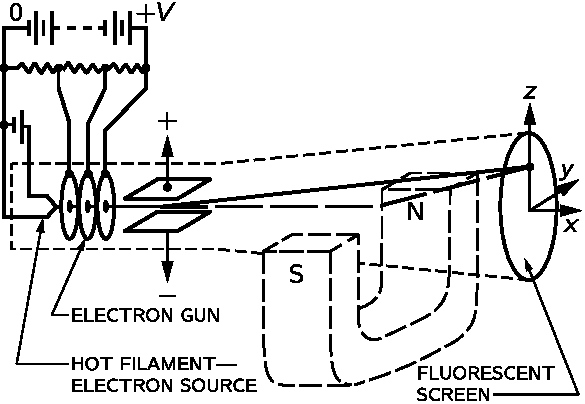
\includegraphics[width=0.8\linewidth]{fyz_fig123.pdf}
      \caption{Obrazovka: 1 - elektronové dělo; 2 - žhavé vlákno - zdroj elektronů; 3 - 
               fluorescenční stínítko 
              (\cite[s.~179]{Feynman01})}
      \label{fyz:fig123}
    \end{figure}
    
    V první částí experimentuje záporné napětí na spodní desce, což znamená, že se na ni přivede 
    více elektronů. Protože souhlasné náboje se odpuzují, světelný bod na stínítku se okamžitě 
    posune nahoru. (Mohli bychom dokonce říci, že elektrony reagovaly na pole tím, že uhnuly směrem 
    nahoru.) Dále změníme napětí, takže zápornou bude \emph{horní} deska. Světelný bod na obrazovce 
    poskočí dolů jako důsledek odpuzování mezi elektrony paprsku a elektrony na horní desce. (Znovu 
    jsme mohli říci, že elektrony zareagovaly na pole, které má nyní opačný směr.)
    
    
    V	druhé části experimentu odpojíme napětí z desek a budeme zkoumat vliv magnetického pole na 
    paprsek elektronů. Použijeme k tomu podkovovitý magnet s dostatečně vzdálenými póly, aby se 
    obrazovka vešla mezi ně. Předpokládejme, že magnet držíme pod obrazovkou v poloze písmena 
    \(U\), s póly směrem nahoru a s částí obrazovky mezi nimi. Vidíme, že jak se od spodu 
    přibližujeme s magnetem, světelný bod se posouvá, řekněme směrem nahoru. Zdá se, že magnet 
    odpuzuje elektronový paprsek. Není to však tak jednoduché, neboť když magnet obrátíme, aniž 
    bychom vyměnili vzájemnou polohu pólů, a k obrazovce se přibližujeme tentokrát shora, světelný 
    bod se posune \emph{nahoru}, takže elektronový paprsek \emph{není} odpuzován, ale naopak, je 
    přitahován. Vraťme magnet do jeho původní polohy \(U\) níže od obrazovky a začněme znovu. Ano, 
    bod je stále posunutý směrem nahoru, nyní však otočme magnet o \SI{180}{\degree} kolem svislé 
    osy, takže bude stále v poloze \(U\), ale póly budou vzájemně vyměněny. Hle, bod nyní poskočí 
    dolů a v této poloze bude i tehdy, kdy magnet převrátíme a přisuneme k obrazovce shora jako 
    předtím.
    
    Abychom pochopili toto divné chování, musíme mít nějakou novou kombinaci sil. Vysvětíme to 
    takto: mezi póly magnetu je \textbf{magnetické pole}. Směr tohoto pole je vždy od jednoho pólu 
    (který si můžeme označit) k druhému. Obrácením magnetu se směr pole nezměnil, ale výměnou pólů 
    se jeho směr změnil. Například, jestliže se elektrony pohybovaly vodorovně ve směru osy \(x\) a 
    i magnetické pole bylo vodorovné ve směru osy \(y\), magnetická síla, působící \emph{na 
    pohybující se elektrony}, měla směr osy \(z\), tj. nahoru nebo dolů, podle toho, zda mělo pole 
    směr kladné nebo záporné osy \(y\).
    
    I když ještě nemůžeme uvést přesný zákon síly mezi navzájem se libovolně pohybujícími náboji, 
    neboť je příliš komplikovaný, uvedeme ho jen v jednom případě: \emph{jsou-li známa pole}. Síla,
    působící na nabité těleso, závisí na jeho pohybu. Je-li těleso v klidu a působí na něho nějaká 
    síla, tato síla je úměrná náboji a koeficient úměrnosti je to, čemu říkáme \emph{intenzita 
    elektrického pole}. Jestliže se těleso pohybuje, síla se může změnit a její korekce, nová 
    přídavná síla, je přesně \emph{lineárně závislá na rychlosti}, působí však pod \emph{pravými 
    úhly} k \(v\) a k druhé veličině, kterou nazýváme \emph{magnetická indukce} \(\vec{B}\). 
    Jestliže složky intenzity elektrického pole \(\vec{E}\) jsou (\(E_x, E_y, E_z\)) a složky 
    magnetické indukce \(\vec{B}\) jsou (\(B_x, B_y, B_z\)) a jestliže složky rychlosti jsou 
    (\(v_x, v_y, v_z\)), pak celková elektrická a magnetická síla působící na pohybující se náboj 
    má tyto složky
    \begin{align}\label{FYZ:eq011}
      F_x &= q(E_x + v_yB_z - v_zB_y)   \nonumber \\ 
      F_y &= q(E_y + v_zB_x - v_xB_z)   \nonumber \\
      F_z &= q(E_z + v_xB_y - v_yB_x)
    \end{align}
    Například, kdyby mělo magnetické pole jen složku \(B_x\) a kdyby byla jedinou složkou rychlosti 
    \(v_x\), pak by měla magnetická síla složku ve směru osy \(z\), pod pravými úhly k \(\vec{B}\) 
    i k \(\vec{v}\).
    
  \section{Nepravé síly}\label{fyz:IchapXIIsecVI}
    Další druh síly, o němž budeme diskutovat, by bylo možné nazvat \textbf{nepravou sílou}; říká 
    se jim též \textbf{síly setrvačné}. V kapitole \ref{fyz:IchapXI} jsme hovořili o dvou 
    lidech, Petrovi a Pavlovi, kteří používali různé souřadnicové soustavy. Nechť polohy částice, 
    které naměří Petr a Pavel jsou \(x\) a \(x'\). Mezi nimi platí
    \begin{equation}\label{FYZ:eq0178}
      x = x' + s, \qquad y=y', \qquad z=z',
    \end{equation}
    kde \(s\) je vzájemné posunutí soustav. Předpokládáme-li, že zákony pohybu platí pro soustavu, 
    v níž se nachází Petr, jak budou vypadat pro soustavu, v níž je Pavel? Nejprve máme
    \begin{equation}\label{FYZ:eq0179}
      \der{x}{t} = \der{x'}{t} + \der{s}{t}.
    \end{equation}
    
    Dříve jsme uvažovali o případu, kdy \(s\) bylo konstantní a zjistili jsme, že \(s\) vůbec 
    neovlivňovalo zákony pohybu, neboť \(ds/dt = 0\). Proto byly v konečném důsledku fyzikální 
    zákony v obou soustavách stejné. Můžeme si však vzít jiný příklad, kdy \(s=ut\), kde \(u\) je 
    rovnoměrná přímočará rychlost. Pak \(s\) není konstanta a \(ds/dt\) není nula, ale je rovno 
    konstantě \(u\). Ale zrychlení \(d^2x/d^2t\) je stále stejné jako \(d^2x'/d^2t\), neboť 
    \(du/dt=0\). To je důkaz principu, který jsme použili v kapitole \ref{chap:fey_hybnost}, že 
    pohybujeme-li se rovnoměrně přímočaře, jsou fyzikální zákony stejné, jako kdybychom byli v 
    klidu. To je Galileova transformace. My si však chceme probrat zajímavý případ, kdy \(s\) je 
    ještě komplikovanější, řekněme, že \(s=at^2/2\). Pak \(ds/dt=at\) a \(d^2s/d^2t = a\), což je 
    \emph{rovnoměrně zrychlený pohyb}. V ještě komplikovanějším případě může být \(a\) obecnou 
    funkcí času. Znamená to, že i když z hlediska Petra budou mít zákony síly tvar
    \begin{align}
      m\dder{x}{t}  &= F_x,        \label{FYZ:eq0180} \\
      \shortintertext{z Pavlova hlediska budou tedy ve tvaru} 
      m\dder{x'}{t} &= F_x - ma,   \label{FYZ:eq0181}
    \end{align}
    
    Protože Pavlova soustava souřadnic se zrychluje s ohledem na Petrův systém, Pavel si bude muset 
    svou sílu opravit o hodnotu \(ma\), jestliže chce, aby byl Newtonův zákon splněn. Jinými slovy, 
    vyskytuje se zde nová tajemná síla neznámého původu, která vzniká z toho důvodu, že Pavel má 
    špatnou soustavu souřadnic. Je to příklad nepravé síly. Další příklady se vyskytují v 
    \emph{rotujících} souřadnicových soustavách.
    
    Jedním z nich je tzv. „odstředivá síla“. Pozorovatel, nacházející se v rotující souřadnicové 
    soustavě, například v otáčející se kabině, objeví tajemnou sílu (kterou nelze vysvětlit na 
    základě žádného známého zdroje síly), jež vrhá předměty směrem ven, ke stěnám. Takové síly 
    existují prostě proto, že pozorovatel se nenachází v newtonovské souřadnicové soustavě, jež je 
    nejjednodušší souřadnicovou soustavou.
    
    Nepravou sílu lze ilustrovat pomocí zajímavého experimentu, při němž po stole posouváme se 
    zrychlením pohár s vodou. Na vodu působí tíha směrem dolů, ale v důsledku horizontálního 
    zrychlení působí na ni i horizontální nepravá síla ve směru opačném ke zrychlení. Výslednice 
    gravitační síly a nepravé síly svírá s vertikálou určitý úhel. Po dobu zrychlování bude povrch 
    vody k této výslednici kolmý. Hladina bude svírat s povrchem stolu stejný úhel, přičemž voda na 
    zadní straně poháru bude vyšší. Když přestaneme posunovat pohár, a ten se v důsledku tření 
    začne zpomalovat, nepravá síla změní svůj směr a voda bude sahat výše na předním okraji poháru 
    (obr. \ref{fyz:fig124}).
    
    \begin{figure}[ht!]  %\ref{fyz:fig124}
      \centering
      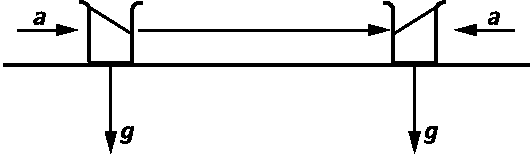
\includegraphics[width=0.7\linewidth]{fyz_fig124.pdf}
      \caption{Ilustrace nepravé síly
              (\cite[s.~181]{Feynman01})}
      \label{fyz:fig124}
    \end{figure}
    Velmi zajímavou vlastností nepravých sil je, že jsou vždy úměrné hmotnostem; totéž platí pro 
    gravitaci. Existuje proto možnost, že i \emph{sama gravitace je nepravou silou}. Není snad 
    možné, aby gravitace existovala prostě proto, že nemáme správnou souřadnicovou soustavu? Konec 
    konců, sílu úměrnou hmotnosti můžeme dostat vždy, když si představíme, že těleso se zrychluje. 
    Například člověk, nacházející se v uzavřené kabině klidně ležící na Zemi, zjišťuje, že je 
    přitahován k podlaze silou úměrnou své hmotnosti. Kdyby ale nebylo Země a kabina by byla v 
    klidu, člověk by se v ní vznášel v prostoru. Na druhé straně, kdyby nebylo Země a kdyby něco se 
    zrychlením \(g\) \emph{zvedalo} kabinu, člověk v kabině by při fyzikální analýze zjistil 
    nepravou sílu, která ho přitlačuje k podlaze, právě tak jako to dělá gravitace.
    
    Einstein vyslovil známou hypotézu, že zrychlení imitují gravitaci, že síly v důsledku zrychlení 
    (tj. nepravé síly) \emph{není možné rozlišit} od gravitačních sil; nelze říci, jakou část z 
    dané síly tvoří gravitace a jakou část tvoří nepravá síla.
    
    Považovat gravitaci za nepravou sílu a říci, že dolů nás přitahuje proto, že jsme urychlováni 
    nahoru, se může zdát správné, ale co potom s lidmi v Austrálii, na druhé straně Země - ti jsou 
    také urychlováni? Einstein objevil, že gravitační sílu lze považovat za nepravou sílu současně 
    jen v jednom bodě a svými úvahami dospěl k názoru, že \emph{geometrie světa je} složitější, 
    než obyčejná euklidovská geometrie. Naše diskuse o problému gravitace je jen kvalitativní a 
    neklade si za cíl nic více, než náčrt základních myšlenek. Abychom aspoň přibližně znázornili, 
    jak může být gravitace výsledkem nepravých sil, uvedeme čistě geometrickou ilustraci, jež 
    neodpovídá reálné situaci. Předpokládejme, že žijeme v dvojrozměrném světě a nic nevíme o 
    existenci třetího rozměru. My si myslíme, že žijeme na rovině, ale nechť to je ve skutečnosti 
    povrch koule. Dále předpokládejme, že podél povrchu vystřelíme nějaké těleso, na které nepůsobí 
    žádné síly. Kam poletí? Bude se zdát, že letí po přímce, ale protože musí zůstat na povrchu 
    koule, kde nejkratší vzdáleností mezi dvěma body je oblouk, hlavní kružnice poletí po tomto 
    oblouku. Vystřelíme-li podobně jiné těleso, ale v jiném směru, poletí podél jiné hlavní 
    kružnice. Protože si myslíme, že žijeme na rovině, budeme očekávat, že dráhy těchto dvou těles 
    se budou od sebe s rostoucím časem lineárně vzdalovat, ale přesným pozorováním zjistíme, že po 
    průletu dost velké vzdálenosti se začnou znovu k sobě přibližovat, jako kdyby se vzájemně 
    přitahovala. Ona se však navzájem nepřitahují - jen geometrie je jaksi „divná“. Tato ilustrace 
    nepopisuje korektně co je „divné“ na euklidovské geometrii, znázorňuje jen to, že když 
    dostatečně pozměníme geometrii, je možné, že celá gravitace nějak souvisí s nepravými silami; a 
    to je základní myšlenka \textbf{Einsteinovy teorie gravitace}.
    
  \section{Jaderné síly}\label{fyz:IchapXIIsecVII}
    Tuto kapitolu uzavřeme krátkou diskuzí o jediných dalších známých silách - \textbf{jaderných 
    silách}. Působí v jádrech atomů, a ačkoli se o nich hodně hovoří, nikdo nikdy ještě nevypočítal 
    sílu působící mezi dvěma jádry. Zákon jaderných sil není v současnosti znám. Tyto síly mají 
    velmi krátký dosah, přibližně takový, jako je rozměr jádra, asi \SI{e-15}{\m}. Pro tak malé 
    částice a na tak malých vzdálenostech platí jen zákony kvantové mechaniky, ne zákony 
    newtonovské. Při analýze atomových jader nepracujeme s představou sil; pojem síly můžeme 
    nahradit pojmem \emph{energie interakce dvou částic}, o čemž si pohovoříme později. Každý 
    vztah, který lze napsat pro jaderné síly, je jen velmi hrubou aproximací, jež zanedbává 
    množství komplikací. Jedním takovým vztahem může být tento: síly v jádře se nemění nepřímo 
    úměrně druhé mocnině vzdálenosti, ale zanikají exponenciálně s \(r\), jak to vyjadřuje vztah
    \begin{equation}\label{FYZ:eq0182}
      F = \frac{1}{r^2}\exp\left(-\frac{r}{r_0}\right),
    \end{equation}
    kde \(r_0\) je rovno vzdálenosti řádu \num {e-15} metru. Tedy síly zmizí, jakmile se částice 
    vzdálí na větší vzdálenost, ačkoli v dosahu \SI{e-15}{\m} jsou velmi silné. Podle současného 
    chápání jsou zákony jaderných sil velmi složité; neznáme jednoduchý způsob, jak je pochopit a 
    celý problém analýzy fundamentálních procesů, jež za nimi stojí, není vyřešen. Pokusy najít 
    řešení vedly k objevům mnoha neobyčejných částic, jako například \(\pi\)-mezonů, ale podstata 
    těchto sil zůstává nejasná\footnote{Právě Feynmanovou zásluhou úsilí o pochopení jaderných sil 
    značně pokročilo; přivedlo například k představě o kvarkovém modelu jaderných částic.}. 
    
%} %tikzset
%---------------------------------------------------------------------------------------------------
\printbibliography[heading=subbibliography]
\addcontentsline{toc}{section}{Seznam literatury}